\section{ER Diagram}
\begin{figure}[H]
  \centering
  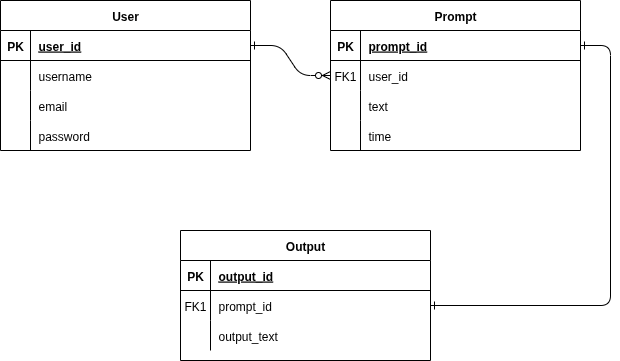
\includegraphics[width=1\textwidth]{images/er_diagram.png}
  \caption{Entity-Relationship Diagram of FormalNet}
  \label{fig:er}
\end{figure}
The Entity Relationship Diagram represents the data model of the FormalNet system. It defines the structure of the database and the relationships between various entities.

In the FormalNet system:
\begin{itemize}
    \item A User can submit multiple Prompts, forming a one-to-many relationship.
    \item Each Prompt is processed by the model, and the corresponding FormalOutput is generated and stored, establishing a one-to-one relationship between Prompt and Output.
    \item Foreign keys maintain referential integrity between the tables
\end{itemize}
This diagram helps in designing an efficient database schema and serves as a foundation for backend development and query optimization.


\section{Dataflow Diagram}
\begin{figure}[H]
  \centering
  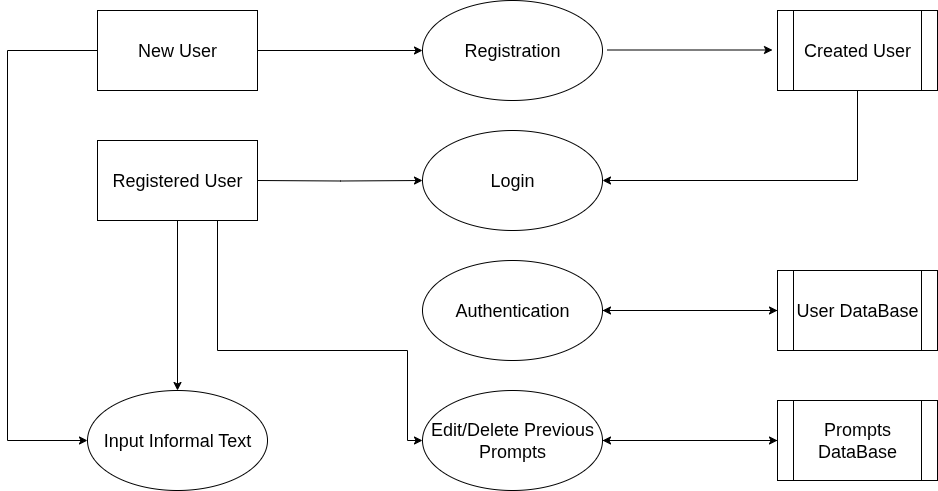
\includegraphics[width=1\textwidth]{images/dataflowdiagram.png}
  \caption{Dataflow Diagram of FormalNet}
  \label{fig:df}
\end{figure}
The data flow diagram (DFD) of the FormalNet system illustrates the movement of data between users, processes, and data stores. It shows how new users register and have their information stored, while registered users can log in and be authenticated using the user database. After authentication, users can input informal text for processing or manage their previous prompts. These actions interact with dedicated databases for storing user and prompt data. The diagram ensures a clear overview of how data flows through the system in a structured manner.


\section{State Diagram}
\begin{figure}[H]
  \centering
  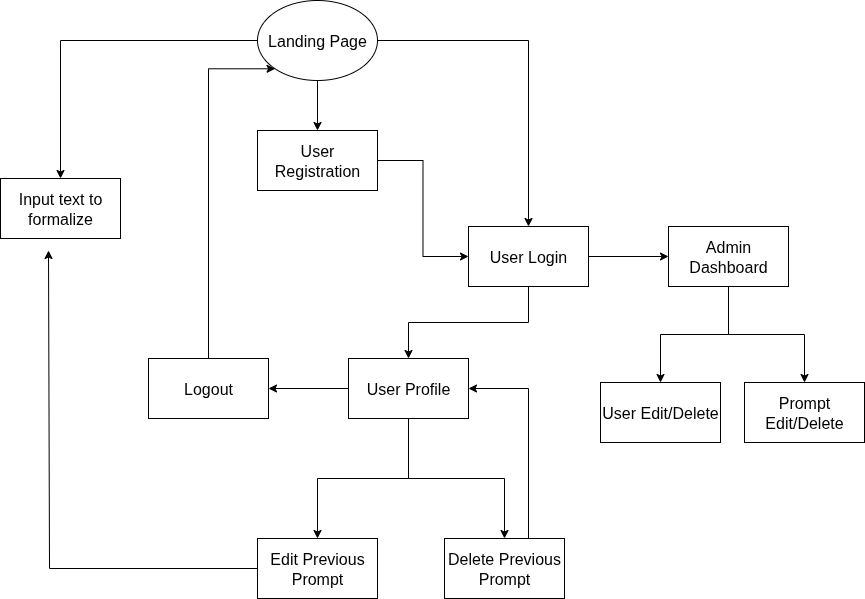
\includegraphics[width=1\textwidth]{images/formalnet state diagram.png}
  \caption{State Diagram of FormalNet}
  \label{fig:statediagram}
\end{figure}
The state diagram of the FormalNet system represents the various states a user or the system can be in during interaction. It begins from the initial state where the user accesses the platform, followed by transitions through states like registration, login, authentication, and text input. Depending on user actions, the system can move to states such as prompt editing or logout. This diagram helps visualize the dynamic behavior of the system and how it responds to different user inputs and transitions.


\section{Use Case Diagram}
\begin{figure}[H]
  \centering
  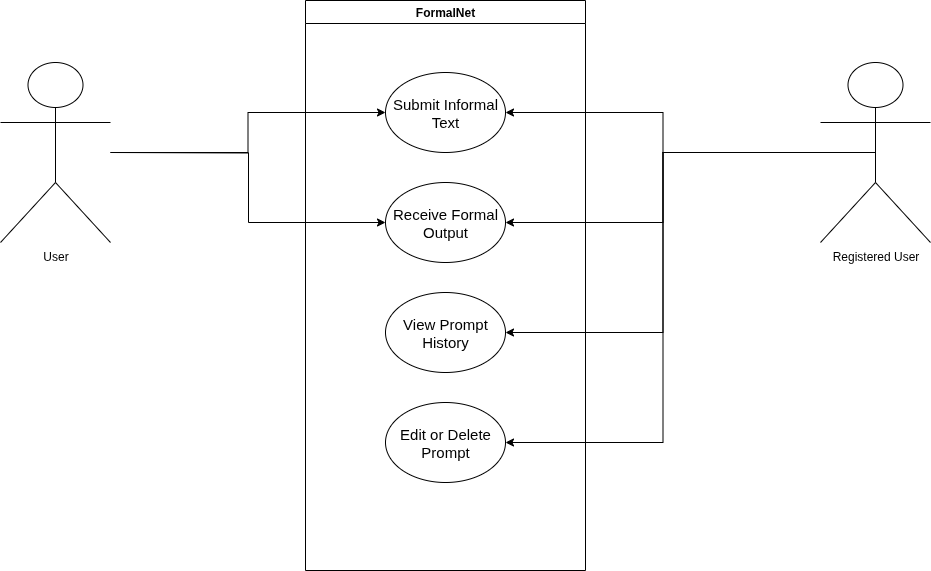
\includegraphics[width=1\textwidth]{images/usecasediagram.png}
  \caption{Use Case Diagram of FormalNet}
  \label{fig:usecase}
\end{figure}
The use case diagram provides a high-level visual representation of the interactions between users (actors) and the system (FormalNet). It outlines the core functionalities that the system offers and the roles that interact with them. This helps in identifying system boundaries and user goals in a clear and concise manner.

There are two main actors in the system:
\begin{itemize}
    \item \textbf{New User}: A user who accesses the system without registration.
    \item \textbf{Registered User}: A user who has an account and can access extended functionalities.
\end{itemize}
The primary use cases shown in the diagram include:
\begin{itemize}
    \item \textbf{Submit Informal Text}: Allows users to input informal text into the system.
    \item \textbf{Receive Formal Output}: The system processes the input and returns a formal version of the text.
    \item \textbf{View Prompt History}: Registered users can view their previous inputs and outputs.
    \item \textbf{Edit or Delete Prompt}: Enables users to manage their past prompts for corrections or updates.
\end{itemize}
This diagram helps in understanding the user interaction flow and serves as a blueprint for system behavior from the user's perspective.